\documentclass[12pt,letterpaper]{article}
\usepackage{amsmath}
\usepackage{amsfonts}
\usepackage{amsthm}
\usepackage{cancel}
\usepackage[margin=1in]{geometry}
\usepackage{titling}
\usepackage{multirow}
\usepackage{amssymb}
\usepackage{graphicx}

\setlength{\droptitle}{-10ex}

\preauthor{\begin{flushright}\large \lineskip 0.5em}
\postauthor{\par\end{flushright}}
\predate{\begin{flushright}\large}
\postdate{\par\end{flushright}}

\title{ECS 160 Homework 1 \vspace{-2ex}}
\author{Hardy Jones\\
        999397426\\
        Professor Levitt\vspace{-2ex}}
\date{Spring 2014}

\begin{document}
  \maketitle

  \begin{enumerate}
    \item We require this additional requirement:

      A book can only be added to the set if it passes the test of the censor.

      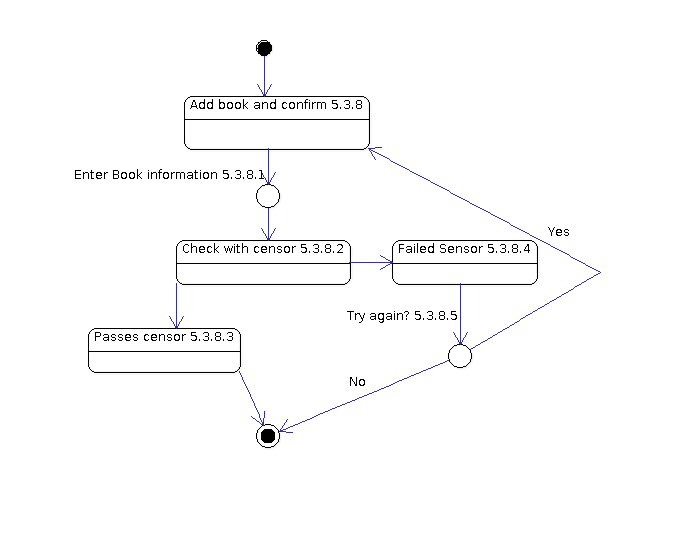
\includegraphics[width=\textwidth]{hw1_part1.png}

    \item For the additional use case ``Apply for an MSG Mortgage''

      The applicants would fill out a form with the couple's information.
      The form would need to request financial details along with home details.
      An MSG employee would then input the information into the system.

      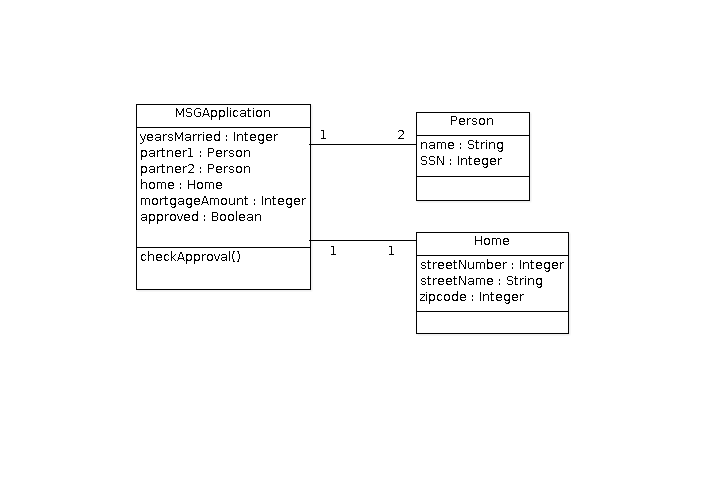
\includegraphics[width=\textwidth]{hw1_part2.png}
      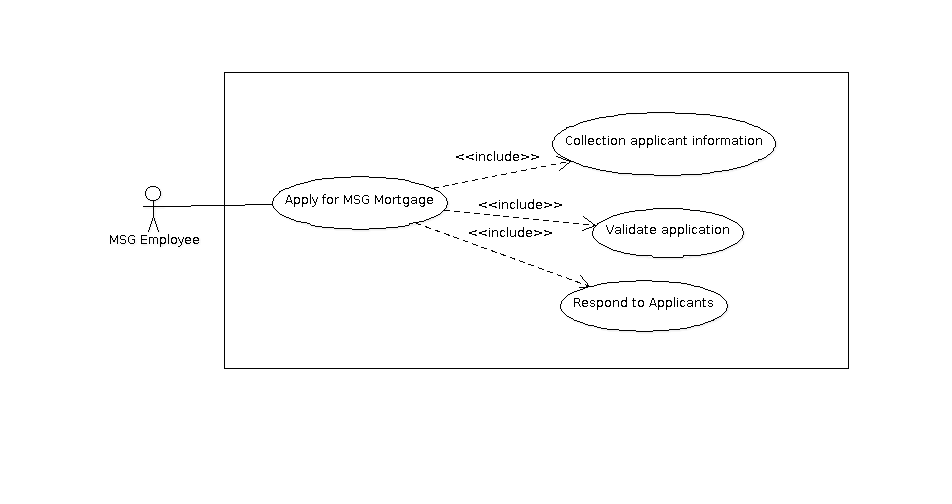
\includegraphics[width=\textwidth]{hw1_part2_2.png}
      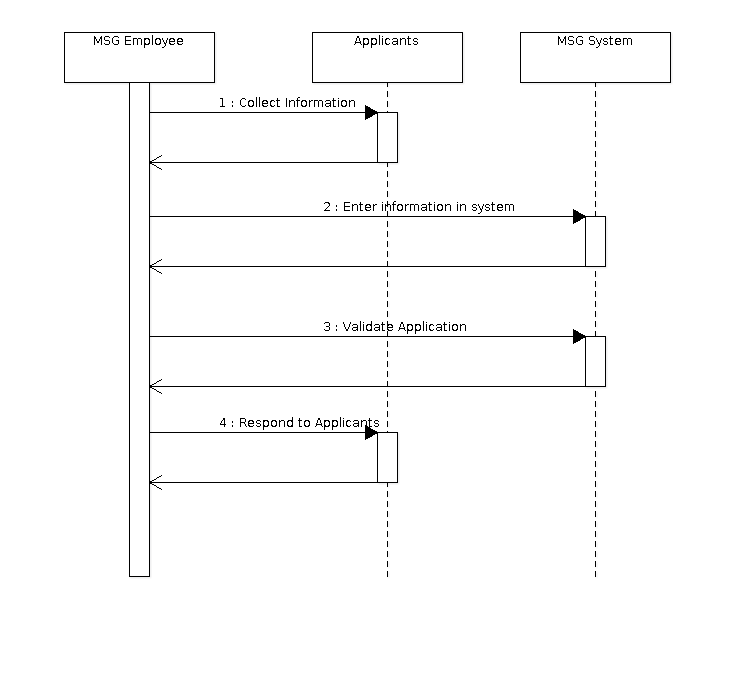
\includegraphics[width=\textwidth]{hw1_part2_3.png}

    \item For the checking system

      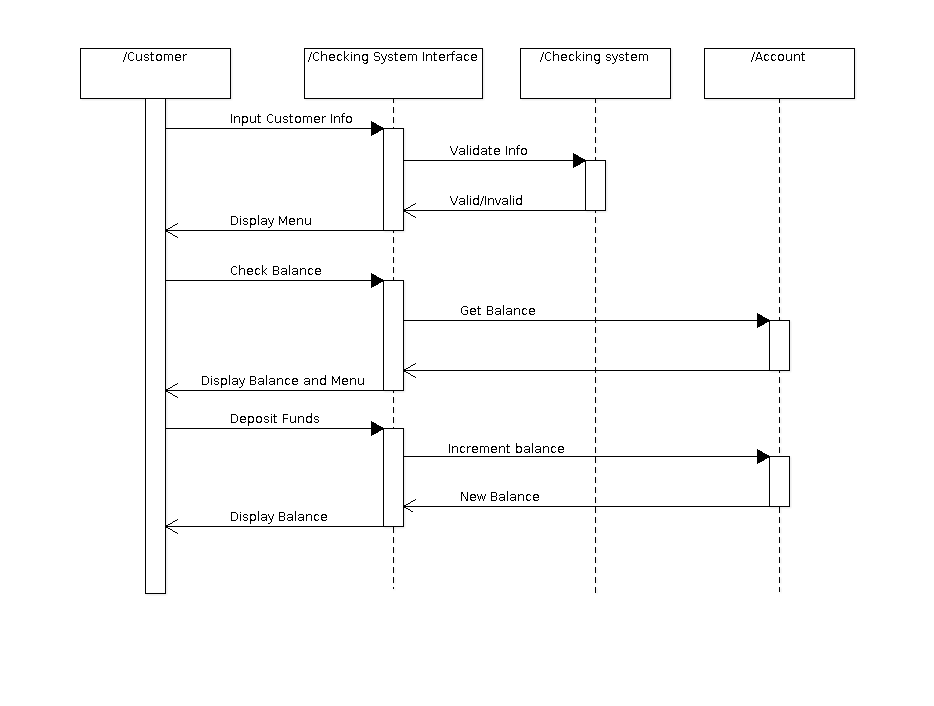
\includegraphics[width=\textwidth]{hw1_part2_4.png}
  \end{enumerate}
\end{document}
